\documentclass[11pt]{article}
\usepackage{acl2014}
\usepackage{times}
\usepackage{url}
\usepackage{latexsym}
\usepackage{graphicx}
\usepackage{adjustbox}
\usepackage{array}
\usepackage{booktabs}
\usepackage{multirow}
\usepackage{multicol}% http://ctan.org/pkg/multicols
\usepackage{tabularx, booktabs}
\usepackage{framed}
\usepackage{setspace} 

% Change this if needed to set titlebox size.
%\setlength\titlebox{5cm}

\title{LING 573: Deliverable 3 Project Report}

\author{Clara Gordon \\
  University of Washington \\
  Seattle, WA \\
  {\tt cgordon1@uw.edu} \\\And
  Claire Jaja \\
  University of Washington \\
  Seattle, WA \\
  {\tt cjaja@uw.edu} \\\And
  Andrea Kahn \\
  University of Washington \\
  Seattle, WA \\
  {\tt amkahn@uw.edu} \\}

\date{}

\begin{document}
\maketitle
\begin{abstract}

In this paper, we describe a question answering system for handling factoid questions.  The system, implemented in Python, follows a typical pipeline, including query processing, information retrieval, and answer candidate extraction and ranking modules. Using the AQUAINT corpus of English News Text as a document collection, it produces answers for questions from the QA track of the Text Retrieval Conference (TREC).

\end{abstract}

\section{Introduction}

Question answering (QA) has long been a prominent problem in the field of natural language processing. In contrast to information retrieval (IR) systems, which return relevant documents based on search terms, a question answering system takes a natural-language question as input and outputs a natural-language answer. IR is typically a component of the system, but the addition of question and answer processing prevents users from having to sift through long documents to find the information they are seeking.

We implemented a question answering system to handle factoid questions from the QA track of the Text Retrieval Conference (TREC), using the AQUAINT Corpus of English News Text as a document collection.

\section{System Overview}

Our system is coded in Python. Third-party modules that we use include Indri/Lemur (for IR), pymur (a Python wrapper for Indri/Lemur), Beautiful Soup (for XML parsing), and NLTK (for tokenization and query expansion). We chose Indri/Lemur for IR because of its specific handling of TREC-formatted question files. We currently use a stopword list taken from the Indri/Lemur documentation.

We use Indri's IndriBuildIndex code to build an index.  It has a parameter file specified as an argument which gives the path to the document collection, the path to the output index, and other parameters.  Indexing of the AQUAINT corpus takes approximately 15 minutes.  We created several different versions of the index for D3, using both Porter and Krovetz stemmers, both including and excluding a list of stopwords.

The core of our system is a three-part pipeline, consisting of modules for question processing, IR, and answer processing, respectively. The system architecture is shown in Figure 1.

\begin{figure}
  \centering
    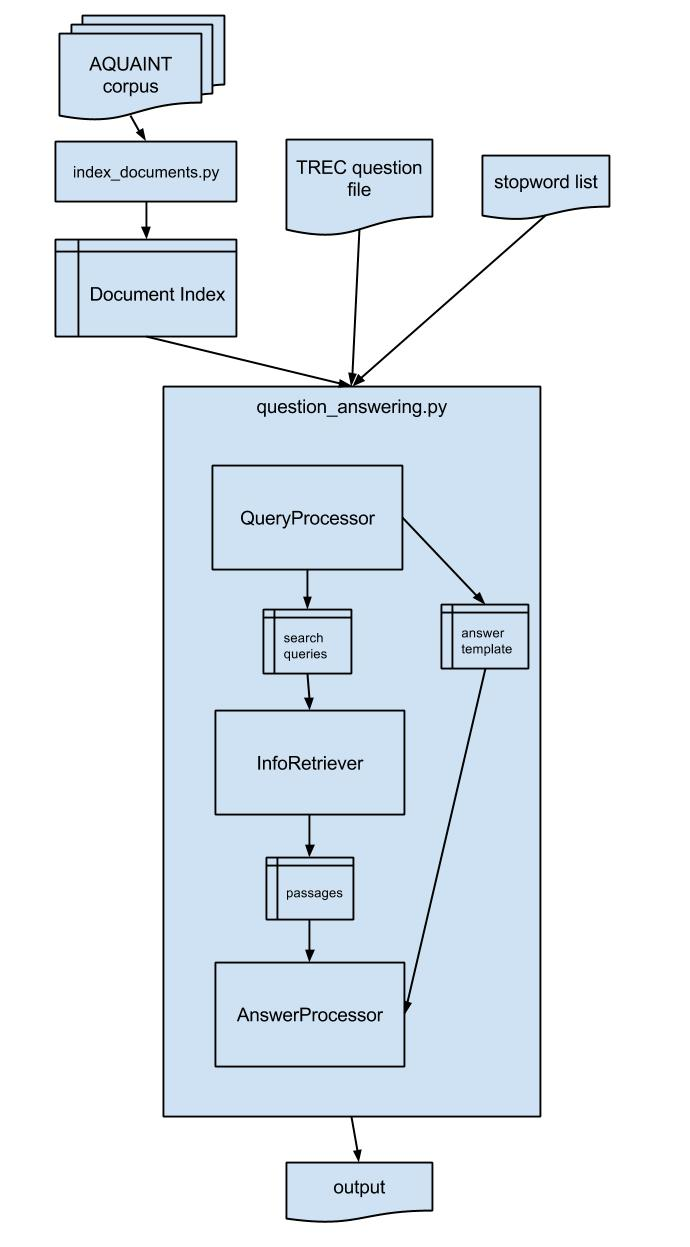
\includegraphics[width=0.5\textwidth]{system_architecture.jpg}
 \caption{System architecture.}
\end{figure}

\section{Approach}

The question answering system is called by a wrapper script, question\_answering.py, which takes as arguments a file containing questions in TREC QA format, a path to the document index, a path to cached web results, a run tag, and a path to the desired output file. It uses the third-party module Beautiful Soup to parse the XML in the TREC document and generate a list of questions. Currently, Python's multiprocessing module is used to parallelize the questions in the question file, so that multiple questions may be passing through the pipeline (described in detail below) at once. For each in the group of answers returned for each question, the wrapper script prints the question ID, the run tag, the document ID associated with the answer, and the answer to the output file.

Classes that are used by multiple modules in the pipeline are defined in the module general\_classes.py. These include:

\begin{itemize}
\item Question class: A Question object stores as attributes the TREC question ID, the question type, the TREC natural-language question stored as a string, and the "target" (the context given for a set of questions in TREC 2004-2006; defaults to None).
\item SearchQuery class: A SearchQuery object stores as attributes a dictionary of search terms, each of which can be one or more words, mapped to weights indicating how important those terms are perceived as being, and an overall weight for the query, which will be used to calculate the probability of the corresponding AnswerCandidate.
\item AnswerTemplate class: An AnswerTemplate object stores as attributes the question ID, a set of basic search query terms from the original question, and a dictionary for the weights of each answer type, where the weights will be used to reweight AnswerCandidate objects during answer processing.
\item Passage class: A Passage object stores as attributes the text of a snippet, its weight, and the document ID.
\end{itemize}

\subsection{System architecture}

Our pipeline for processing a single question consists of three components found in three separate modules, described below. The pipeline takes a Question object as input and outputs a list of AnswerCandidate objects.

\subsubsection{Query processing}

The query processing module is responsible for creating one or more weighted search queries (which are passed to the information retrieval module to be used for passage retrieval) and instantiating an answer template (which is passed to the answer processing module to be used during answer ranking).

A QueryProcessor object is initialized with a Question object and generates a vocabulary, or a list of words (i.e., whitespace-tokenized strings) occurring in the question/target and their counts. We use NLTK's named-entity chunker to remove named entities before tokenizing to prevent the named entities themselves from being tokenized. The named entities are later added back into the query terms when the search queries are generated.

After instantiating a QueryProcessor object, the wrapper script then calls a method in the query-processing module that instantiates an AnswerTemplate object that will subsequently be passed to the answer processing module. The answer template contains the query processor's vocabulary so that the answer processing module can downweight answer candidates that contain query terms. In addition, this method employs regular-expression matching on the original natural-language question to identify questions as requiring an answer that is the name of a person (i.e., proper noun), the name of an organization (i.e., proper noun), the name of an object (i.e., common noun), the name of a location (i.e., proper noun), a time expression, a number expression, or some expression that does not fall into one of these categories. Some regular expressions correspond with one of these answer types; others correspond with multiple answer types. A regular expression match causes the corresponding answer types to be given a higher weight in the AnswerTemplate dictionary of answer type weights. Currently, we set the weights of answer types corresponding with a regular expression that matches to 0.9, weights of all other answer types to 0.1, and the weight of "other" to 0.5 if no regular expression matches. In subsequent versions, we plan to experiment with different weighting schemes.

The query processor is then used to generate a list of weighted search queries, each of which is in turn a set of weighted search terms. In the current version, the query processor generates a single search query that contains the set of words occurring in the question and the question target, with the word counts as weights.

We also implemented query expansion using NLTK's Lin thesaurus corpus and scored\_synonyms method. Our expand\_query method returns a SearchQuery object containing all of the original query terms and their corresponding weights, as well as the top \emph{n} synonyms for each, their weights being the product of the weight of the original term of which they are synonyms and the weight returned by scored\_synonyms. However, our best system does not use this query expansion, as doing this drastically decreased our strict and lenient scores. In subsequent versions of the system, we plan to implement part-of-speech tagging on the query terms; group query terms in Noun, Verb, Adjective, or Other categories; expand terms in the first three categories; and only return synonyms that are in a matching category (since the synonyms returned by NLTK are classified in these three categories).

\subsubsection{Information retrieval}

The information retrieval module uses the Indri/Lemur IR system to retrieve \emph{n} passages for each set of query terms passed to it by the query processing module. Empirical tests show that returning 40 Indri passages provides the best results. We use Base64 conversion for our queries in order to avoid encoding errors with punctuation. Although we use Indri directly to index the document collection, this portion of the system uses the pymur wrapper to run the query and retrieve passage results. We use the given offset indices to retrieve the passage from the original text. Since these indices refer to the stemmed text, however, the passages may be a slightly different window from that selected by Indri. In future work, we plan to expand these offsets to ensure the passage returned contains the text determined by Indri to best match the query.  We are considering using sentence tokenization to extract all sentences overlapping with the passage range, to include all important components and help downstream text processing.

The pymur commands provide the document ID number and document weight. Together with the reconstructed passage text, these are used to construct a Passage object for each passage. 

In addition to document retrieval, we implement web boosting by using cached web results stored before runtime. A separate script, src/cache\_web\_results.py, submits each unprocessed factoid query to Ask.com. We omit any query processing in this portion of the system because we assume Ask.com has its own query processing algorithms which can be best run raw query. The script uses BeautifulSoup to scrape the text snippets associated with each results, and stores them in a text document in the src/cached\_web\_results directory. After comparing results, we have found that three pages of results is optimal. 

During the IR phase of our system, these cached results are retrieved and stored as Passage objects, similar to the AQUAINT oassages. Because initial experiments show that these web snippets are very likely to contain the answer, we weight them similarly to a very high scoring AQUAINT document in our IR framework: log(0.9).  The document ID for these Passage objects is set to None to indicate that these are web snippets, not passages coming from AQUAINT documents.  Together, the AQUAINT and web-based Passage objects are passed on to the answer extraction module. 

\begin{table*} 
    \begin{center}
      \resizebox{\linewidth}{!}{
\begin{tabular}{|*{6}{c|}}
\hline
\textbf{System} & \textbf{stemmer} & \textbf{stoplist with indexing} & \textbf{\# web results pages} & \textbf{Strict} & \textbf{Lenient} \\ \hline
Baseline & Porter & yes & -- & 0.0051 & 0.0289 \\ \hline
1 & Porter & yes & 4 & \textbf{0.0742} & \textbf{0.1257} \\ \hline % experimenting with different stemmers
2 & Krovetz & yes & 4 & 0.0683 & 0.1279 \\ \hline
3 & none & yes & 4 & 0.0610 & 0.1198 \\ \hline
4 & none & no & 4 & 0.0688 & 0.1278 \\ \hline
\end{tabular}}
\vspace{1mm}
\emph{Table 1: Adding web boosting over baseline, with different index parameters.}
\end{center}
\end{table*}

\begin{table*}
\begin{center}
\resizebox{\linewidth}{!}{
\begin{tabular}{|*{6}{c|}}
\hline
\textbf{System} & \textbf{stemmer} & \textbf{\# web results pages} & \textbf{Question Classification} & \textbf{Strict} & \textbf{Lenient} \\ \hline
1 & Porter & 4 & no & \textbf{0.0742} & \textbf{0.1257} \\ \hline % experimenting with different stemmers
6 & Porter & 4 & yes & 0.0614 & 0.1330 \\ \hline % adding question classification
\end{tabular}}
\vspace{1mm}
\emph{Table 2: Adding question classification.}
\end{center}
\end{table*}

\begin{table*}
\begin{center}
\resizebox{\linewidth}{!}{
\begin{tabular}{|*{7}{c|}}
\hline
\textbf{System} & \textbf{stemmer} & \textbf{\# web results pages} & \textbf{expanded query weight} & \textbf{\# of synonyms} & \textbf{Strict} & \textbf{Lenient} \\ \hline
6 & Porter & 4 & -- & -- & \textbf{0.0614} & \textbf{0.1330} \\ \hline % adding question classification
8 & Porter & 4 & 1 & 3 & 0.0331 & 0.0943 \\ \hline % adding question expansion
9 & Porter & 4 & 2 & 3 & 0.0311 & 0.9010 \\ \hline
10 & Porter & 4 & 1 & 1 & 0.0334 & 0.0927 \\ \hline
11 & Porter & 4 & 0.5 & 1 & 0.0340 & 0.0933 \\ \hline
\end{tabular}}

\vspace{1mm}
\emph{Table 3: Adding query expansion.}
\end{center}
\end{table*}

\begin{table*}
\begin{center}
\resizebox{\linewidth}{!}{
\begin{tabular}{|*{5}{c|}}
\hline
\textbf{System} & \textbf{stemmer} & \textbf{\# web results pages} & \textbf{Strict} & \textbf{Lenient} \\ \hline
12 & Porter & 1 & 0.0659 & 0.1215 \\ \hline
14 & Porter & 2 & 0.0641 & 0.1336 \\ \hline
24 & Porter & 3 & \textbf{0.0709} & \textbf{0.1344} \\ \hline % best final results
6 & Porter & 4 & 0.0614 & 0.1330 \\ \hline
16 & Porter & 5 & 0.0620 & 0.1311 \\ \hline
17 & Porter & 6 & 0.0565 & 0.1222 \\ \hline
13 & Porter & 10 & 0.0634 & 0.1152 \\ \hline
\end{tabular}}

\vspace{1mm}
\emph{Table 4: Testing different number of web pages for web caching.}
\end{center}
\end{table*}

\begin{table*}
\begin{center}
\resizebox{\linewidth}{!}{
\begin{tabular}{|*{5}{c|}}
\hline
\textbf{System} & \textbf{stemmer} & \textbf{\# of Indri passages} & \textbf{Strict} & \textbf{Lenient} \\ \hline
26 & Porter & 20 & 0.0782 & 0.1320 \\ \hline
27 & Porter & 30 & 0.0844 & 0.1416 \\ \hline
28 & Porter & 40 & \textbf{0.0868} & \textbf{0.1499} \\ \hline % best final results
29 & Porter & 50 & 0.0839 & 0.1428 \\ \hline
24 & Porter & 100 & 0.0709 & 0.1344 \\ \hline
\end{tabular}}

\vspace{1mm}
\emph{Table 5: Testing different number of passages returned by Indri.}
\end{center}
\end{table*}

\subsubsection{Answer candidate extraction and ranking}

The answer processing module is used to extract and rank answers.  An object of this class is initialized with a list of Passage objects, an AnswerTemplate object, and an optional stopword list.  This object can then generate and rank answers.  This is done in a series of steps.

First, possible answers are extracted from the Passages by generating all unigrams, bigrams, trigrams, and 4-grams from the text of each passage; the score of each of these possible answers is the sum of the retrieval scores of the passage it is found in.  If an n-gram appears multiple times in a passage, the n-gram's score is updated each time the n-gram appears, so a possible answer that appears frequently in a passage is scored higher than one that appears just once in the passage. At the end, a list of AnswerCandidate objects is generated which contains the question ID, a possible answer, its score, the document collection documents it is found in, and the total number of passages it is found in.  Since we believe that the web snippets are more likely to contain the correct answer than the documents from the document collection, each web snippet passage is counted as ten passages; so if a possible answer occurs in two web snippet passages and one document collection passage, it is counted as having been found in 21 (2*10 + 1) passages.

After this, the answer candidates go through a filtering step.  At this step, any answers that start or end with a stopword or standalone punctuation token, or contain any words from the original query (retrieved from the AnswerTemplate) are discarded.  Additionally, any answers that did not appear in at least \emph{n} document collection documents are discarded, and any answers that did not appear in at least \emph{m} total passages are discarded.  We tested a few different thresholds for these values and found the best results with \emph{n} = 1 and \emph{m} = 10 but hope to do more thorough experimentation on this in the future.

Then, a combining step updates the score of each answer to be the current score plus the sum of the scores of the unigram answers contained within it. This prevents unigrams from being the highest ranked answers and instead favors longer answers.

Next, the answers are reweighted.  Regular expressions are used to guess the type of each answer.  Currently, three different categories are captured; 1) person, organization, or location (identified by an answer beginning with a capital letter), 2) time expression (identified by an answer containing month words or a pattern resembling a date), and 3) numbers (identified by digits as well as number words).  Then, the weights from the AnswerTemplate are applied accordingly.  Since person, organization, and location are not distinguished in the answers, the highest weight among these three in the AnswerTemplate is used for any answer identified as being in that category.

Lastly, the answers are ranked by score, and the top 20 are returned.  For each answer generated, one of the document IDs where the n-gram occurred is randomly selected as the source of the answer.  In future development, a more clever method for selecting which document ID to use as the answer source will be employed.

\section{Results}

We evaluated our results using the mean reciprocal rank (MRR) measure with strict and lenient evaluation. We experimented with adding web boosting, using different index parameters, adding question classification, adding query expansion, changing the number of web pages used for web caching, and changing the number of passages returned by Indri.  The results, based on automatic pattern scoring, are shown in Tables 1 - 5 below.  All scores are rounded to four significant digits.  The best results in each table are bolded.


\section{Discussion}

As shown in our results tables, web boosting provides a significant improvement to our system scores.  The index parameters that give us the best results are using the Porter stemmer and a stoplist.  Adding question classification helps our lenient score but actually results in a decrease in the strict score. (We expect that this is most likely due to the way that the answer types are weighted and the answer-processing module makes use of these weights, and that adjusting these components in future versions may lead to better strict scores with question classification than without.)  Query expansion has a negative impact on the results, across all the query weights and number of synonyms tested (most likely due to the fact that we are not controlling for correct part-of-speech in the expanded synonyms; again, we hope to adjust this in future versions).  It appears that using three pages of web results gives the best results.  Using 40 passages from Indri boosts the results, over using fewer or more passages.

Our best results are from the system using a Porter-stemmed index with a stopword list, question classification, three pages of web search results, and 40 passages returned by Indri.  Our strict score for this system is 0.0868 and our lenient score is 0.1499.

\section{Conclusion}

We implemented a baseline question answering system to handle factoid questions from the TREC QA shared task using the AQUAINT Corpus as a document collection. Thus far, web boosting has provided the biggest improvement in our system. In future development, we plan to experiment with different methods of using the web snippets, try weighting named entity query terms higher, and implement new and improved methods for question classification and query expansion, in the hope of improving our results further.

\nocite{*}
\bibliographystyle{acl}
\bibliography{references}

%\begin{thebibliography}{}

%\end{thebibliography}

\end{document}

